\subsection{Nonlinearity Experiments}
\begin{algorithm}[t]
  \caption{The \emph{wave layer} pseudocode}\label{alg:ch6:wavelayer}
\begin{algorithmic}[1]
  \Procedure{WaveLayer}{$x$}
  \State $u_{lp},\ u_{1} \gets \DTCWT(x, \mbox{nlevels}=1) $ 
  \State $v_{lp},\ v_{1} \gets G(u_{lp},\ u_{1}) $ \Comment{the normal wave gain layer}
  \State $w_{lp} \gets \sigma_{lp}(v_{lp})$ \Comment{lowpass nonlinearity}
  \State $w_{1} \gets \sigma_{bp}(v_{1})$ \Comment{bandpass nonlinearity}
  \State $y \gets \DTCWT^{-1}(w_{lp},\ w_{1})$
  \State $x \gets \sigma_{pixel}(y)$ \Comment{pixel nonlinearity}
  \State \textbf{return} $x$
\EndProcedure
\end{algorithmic}
\end{algorithm}
Taking the same `gain1\_2\_3' architecture used for CIFAR-100, we expand the
\emph{wave gain layer} into one bigger layer
dubbed the \emph{wave layer}, described in \autoref{alg:ch6:wavelayer}. In the wave
layer, we have 3 different nonliearities: the pixel, the lowpass 
and the bandpass nonlinearity.

For these experiments, we test over a grid of possible options for these three
functions:
\begin{table}[h!]
  \centering
\begin{tabular}{l l l l l l l}
  \toprule
  Nonlinearity & \hphantom{abc} & \multicolumn{4}{l}{Values} \\
  \midrule
  Pixel && None & BN+ReLU \\
  Lowpass && None & ReLU & BN+ReLU & $\mathcal{S}$ \\
  Bandpass && None & ReLU & BN+MagReLU & $\mathcal{S}$ 
  \\\bottomrule
\end{tabular}
\end{table}

Where:
\begin{itemize}
  \item `None' means no nonlinearity -- $\sigma(x) = x$.
  \item `BN+ReLU' is batch normalization and ReLU (applies only to real valued
    activations) e.g. \eqref{eq:ch6:bnrelu_lp}.
  \item `ReLU' is a ReLU without batch normalization. Can be applied to the real
    and imaginary parts of a complex activation independently i.e.
    \eqref{eq:ch6:relu_bp}. See \autoref{sec:appE:complex_relu} for equations
    for the passthrough gradients for this nonlinearity.
  \item `BN+MagReLU' applies batch normalization to the magnitude of complex
    coefficients and then makes them strictly positive with a ReLU. This action
    is defined in \eqref{eq:ch6:magrelu_bp}. See \autoref{sec:appE:bnrelu} for
    information on the passthrough and update equations for this nonlinearity.
  \item $\mathcal{S}$ is the soft thresholding of \eqref{eq:ch6:relu_st2}
    applied to the magnitudes of coefficients.  See
    \autoref{sec:appE:soft_shrink} for information on the passthrough and update
    equations for this nonlinearity.
    % We choose a
    % conservative sparsity level of 0.2 (20\% of coefficients set to 0) for these
    % thresholds. A full grid search over
    % sparsity levels would be beneficial, but setting it low initially allows us
    % to test its plausibility as a nonlinearity.
\end{itemize}

\begin{table}[t]
  \renewcommand{\arraystretch}{1.2}
  \small
  \centering
  \def \mywidth {1.4cm}
  \mycaption{Different Nonlinearities in the Gain Layer}{Top-1 Accuracies for
  the `gain1\_2\_3' network trained on CIFAR-100 using different wavelet and pixel nonlinearities.
  The rows of the table correspond to different bandpass nonlinearities and the
  columns correspond to different lowpass nonlinearities.
  $\sigma_{pixel}=\sigma_{lp}=\sigma_{bp}=\text{None}$ is a linear system (with
  max pooling). $\sigma_{pixel}=\F{ReLU},\ \sigma_{lp}=\sigma_{bp}=\text{None}$
  is the system used in earlier experiments, which is linear in the wavelet
  domain and has a nonlinearity in the pixel domain.
 % Results are averages over 3 runs.
  The best result is highlighted in bold corresponding to
  $\sigma_{pixel} = \F{None}$, $\sigma_{lp} = \F{ReLU}$ and $\sigma_{bp} =
  \F{BN+ReLU}$.}
  \label{tab:ch6:nonlinearities}
  \subfloat[$\sigma_{pixel} = \text{None}$]{%
  \label{tab:ch6:nonlinearities1}
  \centering
  \makebox[\textwidth][c]{
  \begin{tabular}{l |p{\mywidth} p{\mywidth} p{\mywidth} p{\mywidth} p{\mywidth} }
      \toprule
      \diagbox[width=3cm]{$\sigma_{bp}$}{$\sigma_{lp}$}& None & ReLU & BN+ReLU & $\mathcal{S}$ \\
      \hline
      None & 45.0 & 63.8 & 64.8 & 61.9 \\
      ReLU & 42.6 & 62.8 & 63.9 & 61.3 \\
      BN+MagReLU & 48.5 & \textbf{65.3} & 64.6 & 62.9 \\
      $\mathcal{S}$ & 44.6 & 63.9 & 63.6 & 61.7 \\
      \bottomrule
    \end{tabular}
  }}\newline
  \subfloat[$\sigma_{pixel} = \F{BN+ReLU}$]{
  \label{tab:ch6:nonlinearities2}
  \centering
  \makebox[\textwidth][c]{
  \begin{tabular}{l |p{\mywidth} p{\mywidth} p{\mywidth} p{\mywidth} p{\mywidth} }
      \toprule
      \diagbox[width=3cm]{$\sigma_{bp}$}{$\sigma_{lp}$}& None & ReLU & BN+ReLU & $\mathcal{S}$ \\
      \hline
      None & 62.8 & 60.7 & 64.2 & 63.0 \\
      ReLU & 62.5 & 60.3 & 64.2 & 63.2 \\
      BN+MagReLU & 64.9 & 61.6 & 64.7 & 65.2 \\
      $\mathcal{S}$ & 63.3 & 60.9 & 63.9 & 63.3 \\
      \bottomrule
    \end{tabular}
    }}
\end{table}


As the pixel nonliearity has only two options, the results are best displayed as
a pair of tables, firstly for no nonlinearity and secondly for the
the standard batch normalization and ReLU. See
\autoref{tab:ch6:nonlinearities} for these two tables. 

Digesting this information gives us some useful insights: 
\begin{enumerate}
  \item It is possible to improve on the gainlayer from the previous experiments
    with the right nonlinearities. The previous section's gain layer corresponds
    to $\sigma_{lp} = \sigma_{bp} = \F{None}$ and $\sigma_{pixel} = \F{ReLU}$, or
    the top left entry of \autoref{tab:ch6:nonlinearities2}.
  \item Doing a ReLU on the real and imaginary parts of the bandpass
    coefficients independently (the second row of both tables) almost always
    performs worse than having no nonlinearity (first row of both tables).
  \item The best combination is to have batch normalization and a ReLU applied
    to the magnitudes of the bandpass coefficients and batch norm and a ReLU
    applied to either the lowpass or pixel coefficients with no nonlinearity in
    the pixel domain.
\end{enumerate}

The best accuracy score of $65.3\%$ is now $0.1\%$ lower than the fully
convolutional architecture, an improvement from the $62.8\%$ score achieved with
only a pixel nonlinearity.

\subsection{Ablation Experiments with Nonlinearities}
Now that we have found the best nonlinearity to use for the \emph{wave layer},
will this improve our ablation study from \autoref{sec:ch6:ablation}? To test this, 
we repeat the
same experiment on CIFAR-100 only, but use the \emph{wave layer} described in
\autoref{alg:ch6:wavelayer}, with $\sigma_{pixel} = \F{None},\ \sigma_{lp} =
\F{ReLU},\ \text{and } \sigma_{bp} = \F{BN+ReLU}$.

See \autoref{fig:ch6:nonlinear_ablation} for the results from these experiments.
When we use the wavelet based nonlinearities, the results change considerably. 
We see an improvement by $1\%$ when the first layer in the CNN is
changed for a wave layer, but any other changes degrade performance.

\begin{figure}[tb]
  \centering
  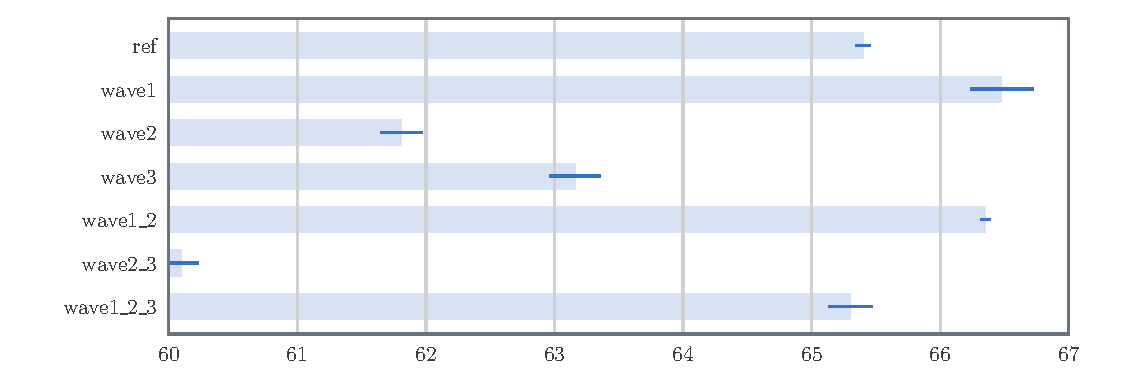
\includegraphics[width=\textwidth]{\imgpath/nonlinear_ablation.pdf}
  \mycaption{CIFAR-100 Ablation results with the \emph{wave layer}}{We use the
  same naming scheme from \autoref{sec:ch6:ablation} but to differentiate
  between the results from \autoref{fig:ch6:cifar100_gl} we call the options
  `waveX' (for \emph{wave layer} vs \emph{gain layer}). When we add
  nonlinearities in the wavelet domain, the ablation results 
  change dramatically. It appears that learning in
  the wavelet domain works best for the first layer of the CNN (wave1), and this
  improves on the purely convolutional method by a whole percentage point.
  Replacing the second and third layers degrades performance independently of
  what was used in the first layer. Swapping the first two layers (wave1\_2)
  performs nearly as well and with a narrower spread.}
  \label{fig:ch6:nonlinear_ablation}
\end{figure}

